\section{Experimental Results}

\label{sec:experiment}


We evaluate 12 advanced LLMs on \textsc{TIDE-Bench}. We report model accuracy across the three sample types, diagnose where chain ambiguity and intent drift individually fail, and examine their interaction when both patterns co-occur in a single dialogue. This analysis distinguishes recognition from resolution and reveals how errors propagate across dialogue phases into their final SQL predictions.


\subsection{Overall Performance}
\label{subsec:performance}

Table~\ref{tab:dea} reports DEA across the three sample types. Performance is low throughout: even the strongest evaluated model, Claude-Sonnet-4.6, reaches only 45.1\% on Drift-only and drops to 27.8\% on Joint, and no model exceeds 46\% overall on any sample type. DEA is consistently highest on Drift-only, lowest on Joint, and intermediate on Chain-only.

This consistently low performance is not concentrated in any particular model class. Larger evaluated models outperform smaller by only 2--3 percentage points on average across three conditions, and the spread between top and bottom models stays within roughly 10 percentage points everywhere. The overall low performance therefore appears to come less from overall model scale than from how agents handle chain ambiguity and user intent drift. The following analyses separate these errors into chain identification, drift recognition, and drift resolution across models and subtypes, and examine how they compound in Joint samples.

\begin{figure*}[!t]
  \centering
  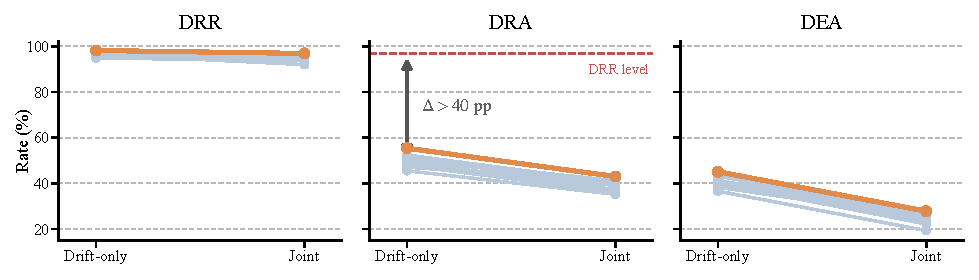
\includegraphics[width=\textwidth]{figure/drift_slope.pdf}
  \vspace{-6mm}
  \caption{Drift handling from Drift-only to Joint across DRR, DRA, and DEA, with one line per model. DRR remains high and flat, while DRA and DEA start lower and decline further in Joint. The dashed DRA reference marks DRR, highlighting the recognition--resolution gap that persists for all models across both interaction settings. The orange line highlights Claude-Sonnet-4.6, which achieves the highest DEA in both Drift-only and Joint.}
  \label{fig:slope}
  \vspace{-2mm}
\end{figure*}


\subsection{What Makes Chain Challenging}
\label{subsec:chain-bottleneck}

\noindent\textbf{Layer-level identification.}
Resolving a chain-only sample requires recognizing dependent clarification layers from the initial question. We measure this directly through per-layer identification rates, with per-model details in Table~\ref{tab:chain-identification} (Appendix~\ref{app:chain-id}). JIR stays below 5\% for every model and below 2\% for the majority, \textbf{\textit{showing that no evaluated model reliably surfaces both clarification layers}}. L1-IR ranges from 5.6\% (Claude-Sonnet-4.6) to 36.2\% (Qwen2.5-72B), with most models clustered in the 20--30\% range, despite L1 being directly available in the initial question. One plausible explanation for the even lower JIR is that L1 difficulty cascades downward: when L1 is missed, the agent may never reach L2 at all. The $p$-protocol (\S~\ref{subsec:interaction}) is designed to remove exactly this confound, pre-populating L1 with its canonical resolution so that L2 is isolated as the sole downstream identification target. Figure~\ref{fig:chain}(a) contrasts L1-IR under the $f$-protocol with L2-IR$^p$ under the $p$-protocol for each model. Even with L1 externally resolved, L2-IR$^p$ ranges only from 1.2\% (Gemini-2.5-Flash) to 13.8\% (Claude-Sonnet-4.6), with half the models still below 10\%, \textbf{\textit{showing that L2 identification fails on its own terms rather than as a side effect of L1 difficulty}}.

\begin{figure}[t]
  \centering
  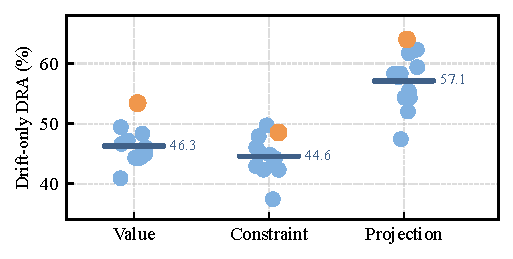
\includegraphics[width=\columnwidth]{figure/drift_subtype_dra.pdf}
  \vspace{-5mm}
  \caption{Drift-only DRA by drift subtype. Points denote models, and the bar marks the corresponding subtype mean. Orange points mark per-subtype maxima.}
  \label{fig:subtype}
  \vspace{-5mm}
\end{figure}

\namedpara{Ask behavior.}
Could this low identification simply reflect how agents ask? An agent that rarely asks for clarification at all, or one that asks freely without targeting genuine ambiguity, would both depress identification rates. Figure~\ref{fig:chain}(b) plots JIR against ask rate (AR) for all 12 models. Ask rates vary widely, ranging from below 10\% to over 60\%, yet JIR stays under 4\% across the entire range. \textbf{\textit{Models that ask more do not surface the chain more reliably}}. Claude-Sonnet-4.6 and Qwen2.5-72B illustrate the two extremes: Claude asks on only 9.7\% of Chain-only samples but Qwen2.5-72B asks on 60.1\%, yet their JIR are at most 1.2\% (0.6\% and 1.2\% respectively). To further isolate whether high asking is selective or indiscriminate, we measure the ask rate on Drift-only samples, where the initial user question carries no chain ambiguity, so any clarification reflects asking that is not ambiguity-driven. Claude's Drift-only ask rate (Table~\ref{tab:chain-identification}) drops to 0.4\%, while Qwen2.5-72B's remains 20.0\%, confirming opposite ask styles. \textbf{\textit{Whether an agent asks selectively or indiscriminately, the chain remains unidentified, pointing to identification capacity itself as the bottleneck}}.

\subsection{Where Drift Handling Fails}
\label{subsec:drift-bottleneck}

\noindent\textbf{Recognition--resolution gap.}
While chain failure is primarily an identification problem, drift exhibits a different failure pattern. We measure whether agents register the drift turn (DRR) and whether they recover an executionally correct post-drift SQL afterward (DRA). Figure~\ref{fig:slope} presents both metrics, with per-model values in Appendix~\ref{app:chain-id}. DRR is at least 94.9\% across models, while DRA remains roughly within the 45--55\% band, \textbf{\textit{leaving every evaluated model with a gap exceeding 40 percentage points between recognizing the drift and successfully resolving user's revised request}}.


\begin{table}[!t]
\centering
\footnotesize
\linespread{1.05}\selectfont
\renewcommand{\arraystretch}{1.2}
\begin{tabularx}{\linewidth}{@{}>{\raggedright\arraybackslash}X@{}}
\toprule

\casehead{Context}\par
\vspace{2pt}
\textit{Schema:}
\texttt{coaches(coachID, year, tmID, won, lost)};
\texttt{teams(year, tmID, won, lost)}.\par
\textit{Question:}
``Which coaches had disappointing seasons in 2000--2010?
Show their coach ID, team, and year.''
\\

\midrule

\casehead{Chain Ambiguity}\par
\vspace{2pt}
\textit{Gold path:}
$L1$: overall losing record
$\rightarrow$
$L2$: team's full-season record.\par
{\color{black!60}
\textit{Alternatives:}\ 
\mbox{$L1$: away-game record;}\ 
\mbox{$L2$: coach-stint record.}}
\\

\addlinespace[2.5pt]
\sqlbox{Gold SQL:}{SELECT DISTINCT c.coachID, t.tmID, c.year FROM coaches c JOIN teams t ON c.tmID=t.tmID AND c.year=t.year WHERE c.year BETWEEN 2000 AND 2010 AND t.lost>t.won}
\\

\addlinespace[3pt]
\textbf{Claude-Sonnet-4.6:} Clarifies that ``disappointing'' means a losing record, but uses
\sql{coaches.lost>coaches.won} without asking whose record should
define the season.\par
\vspace{1pt}
{\scriptsize
\color{black!60}
$L1$ recognized
\quad
$L2$ missed
\quad
\textcolor{red!75!black}{preEX=False \ding{55}}}
\\

\addlinespace[2.5pt]
\textbf{Llama-3.3-70B:}
Also resolves the losing-record interpretation, but applies
\sql{coaches.lost > coaches.won} despite joining \texttt{teams}.\par
\vspace{1pt}
{\scriptsize
\color{black!60}
$L1$ recognized
\quad
$L2$ missed
\quad
\textcolor{red!75!black}{preEX=False \ding{55}}}
\\

\midrule

\casehead{User Intent Drift}\,
{\scriptsize\color{black!60}(constraint-remove)}\par
\vspace{2pt}
Drift utterance: ``Do not limit it to 2000--2010; show those coaches for all years.''
\\

\addlinespace[2.5pt]
\sqlbox{Gold post-drift SQL:}{SELECT DISTINCT c.coachID, t.tmID, c.year FROM coaches c JOIN teams t ON c.tmID=t.tmID AND c.year=t.year WHERE t.lost>t.won}
\\

\addlinespace[3pt]
\textbf{Claude-Sonnet-4.6:}
Removes the year predicate but retains the coach-stint criterion.\par
\vspace{1pt}
{\scriptsize
\color{black!60}
\textcolor{green!50!black}{DRR=True \ding{51}}
\quad
chain error inherited
\quad
\textcolor{red!75!black}{postEX=False \ding{55}}}
\\

\addlinespace[2.5pt]
\textbf{Llama-3.3-70B:}
Makes the same drift update while retaining the same chain error.\par
\vspace{1pt}
{\scriptsize
\color{black!60}
\textcolor{green!50!black}{DRR=True \ding{51}}
\quad
chain error inherited
\quad
\textcolor{red!75!black}{postEX=False \ding{55}}}
\\

\bottomrule
\end{tabularx}

\caption{A \textsc{TIDE-Bench} Joint example. Both models resolve $L1$ but miss the dependent record scope at $L2$; the resulting error persists after a correctly handled drift. SQL and model turns are abridged for space and clarity.}

\label{tab:case-study}
\vspace{-5mm}
\end{table}

\namedpara{Resolution across subtypes.}
To localize this gap, we decompose Drift-only DRA by drift subtype. Figure~\ref{fig:subtype} shows that resolution difficulty is not uniform across the three subtypes defined in \S~\ref{subsec:drift}: a consistent ordering emerges across models where projection-level drift is the easiest to resolve for 11 of 12 models and constraint-level drift is the hardest for 10 of 12, indicating that the resolution gap is structured rather than evenly distributed. The spread is also substantial: within a single model, the subtype-level DRA can differ by as much as 19.4 percentage points (GPT-5.4: projection 61.7\%, constraint 42.3\%). This ordering runs against what SQL complexity alone would predict. Constraint-level drift yields the \emph{simplest} post-drift SQL among the three subtypes, removing only WHERE predicates while leaving join, aggregation, and subquery structure unchanged (Appendix~\ref{app:complexity}). \textbf{\textit{The subtype that yields the simplest SQL is the hardest to resolve, indicating that what makes constraint-level drift difficult is not the SQL itself but inferring which prior commitment is now being retracted}}.

\subsection{How Chain and Drift Interact}
\label{subsec:interaction-finding}

What happens when chain and drift co-occur? Comparing Drift-only to Joint isolates the cost of placing the same drift after a chain phase, with the post-drift ground-truth SQL held identical across the two conditions by construction (\S~\ref{subsec:paired-factorial}). Figure~\ref{fig:slope} traces the shift from Drift-only to Joint across metrics. \textbf{\textit{The drop is asymmetric across all 12 models: DRR shifts by at most 5 percentage points, DRA falls by 6--12, and DEA by 13--18}}. Recognition depends only on the drift turn and is largely unaffected by upstream events; resolution and execution depend on the agent state when the drift arrives. If chain and drift failed independently, Joint DEA would equal the product of Chain-only and Drift-only accuracies, approximately 13\%. Across models, Joint DEA exceeds this prediction by 10--13 percentage points, \textbf{\textit{indicating that the samples on which the two failures occur largely overlap}}.

Across all three analyses, chain ambiguity, user intent drift, and their interaction emerge as three distinct dialogue-level failure modes that current models do not yet handle consistently and reliably.






